\documentclass{article}
\usepackage[utf8]{inputenc} % para que nos acepte la codificación UTF-8
\usepackage[spanish]{babel} % establecemos el idioma del documento al español
\usepackage{graphicx,float}

\begin{document}
\title{Practica 3. Modelos de Computación}
\author{Pablo Navarro}
\maketitle
\begin{enumerate}
  \item Construir un AFND capaz de aceptar una cadena u∈{0,1}*:
  \begin{itemize}
    \item Que comience con la subcadena 011.
    \item Que contenga la subcadena 011.
    \item Que contenga, simultáneamente, las subcadenas 011 y 100. Este AFND
          también acepta cadenas en la que estas subcadenas están solapadas
    \begin{figure}[H]
      \centering
      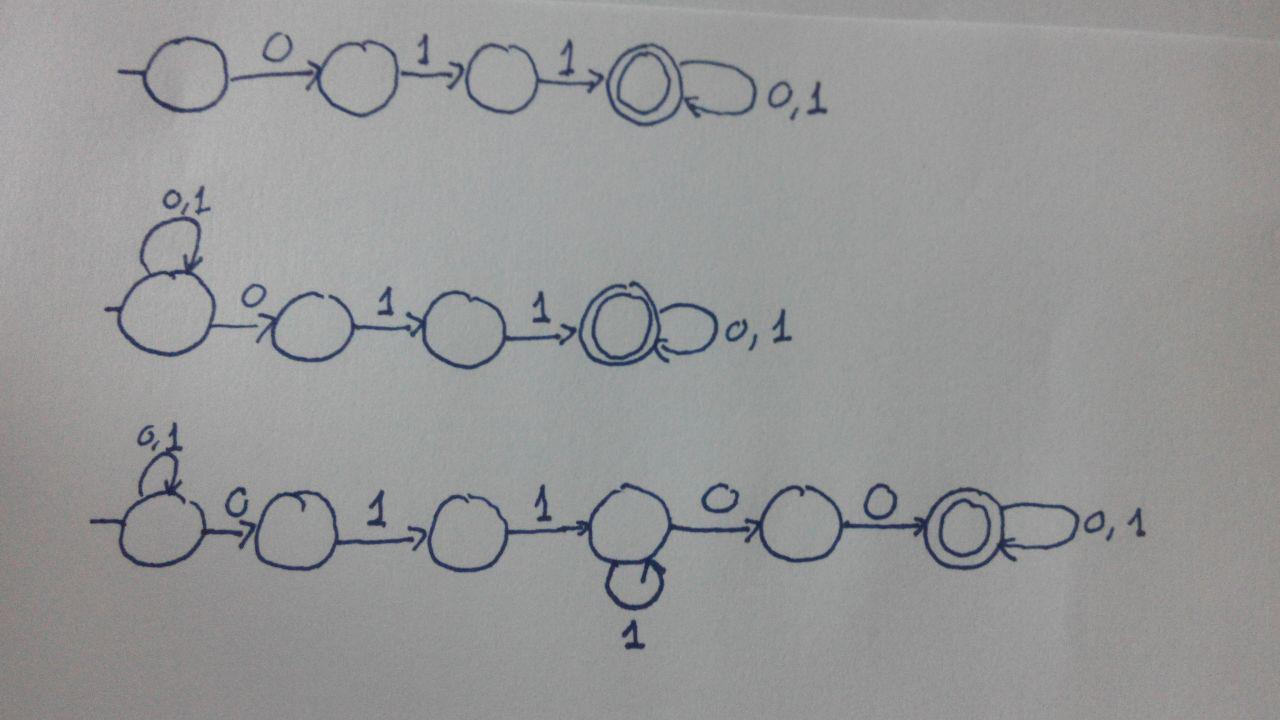
\includegraphics[width=7cm, height=5cm]{imagenes/ejercicio1.jpg}
    \end{figure}
  \end{itemize}
  \item Convertir el AFND a AFD
    \begin{figure}[H]
      \centering
      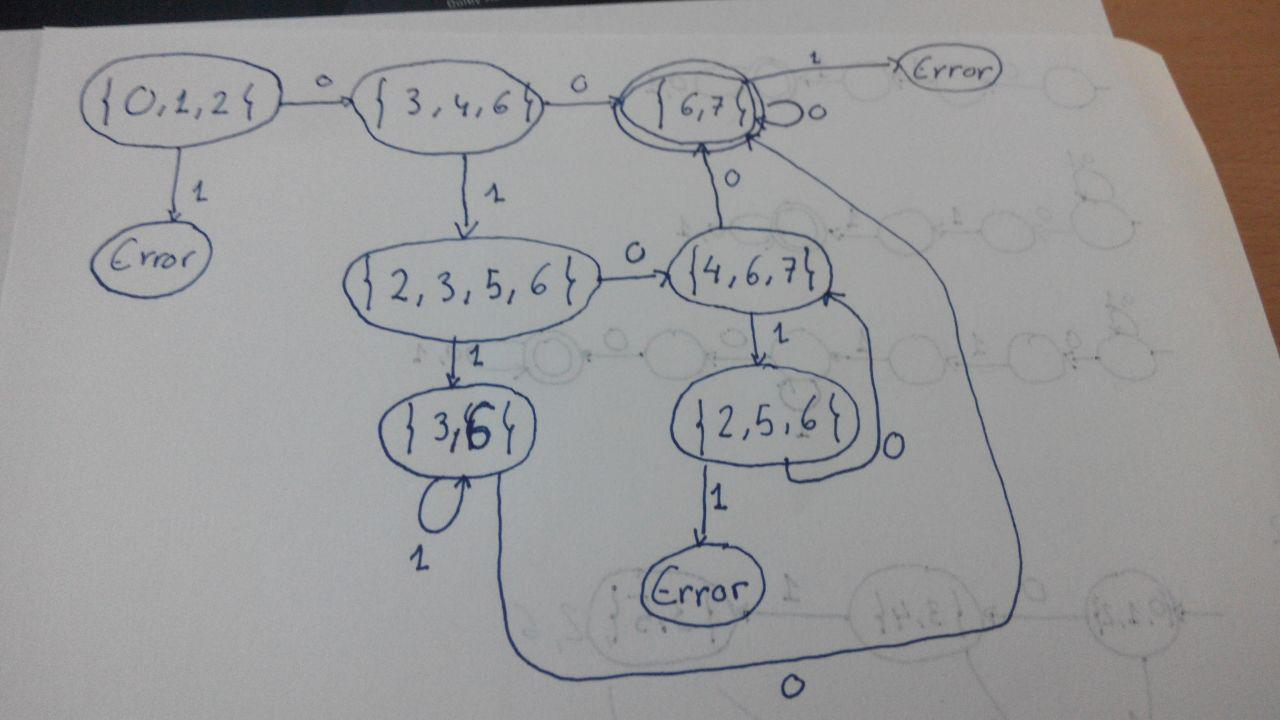
\includegraphics[width=10cm, height=5cm]{imagenes/ejercicio2.jpg}
    \end{figure}
  \item Construir los siguientes AFDs
  \begin{itemize}
    \item $(ab)^*b^*$
    \begin{figure}[H]
      \centering
      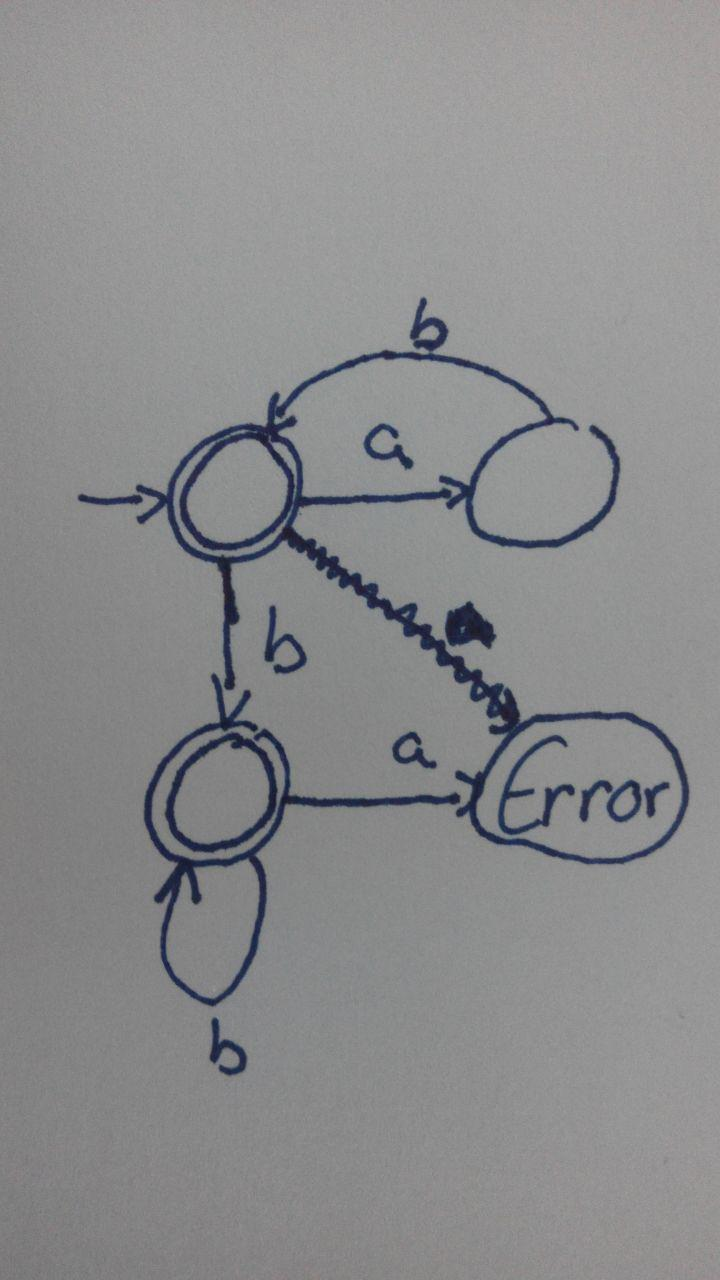
\includegraphics[width=4cm, height=6cm]{imagenes/ejercicio3a.jpg}
    \end{figure}
    \item $(bb^*a)^*b$
    \begin{figure}[H]
      \centering
      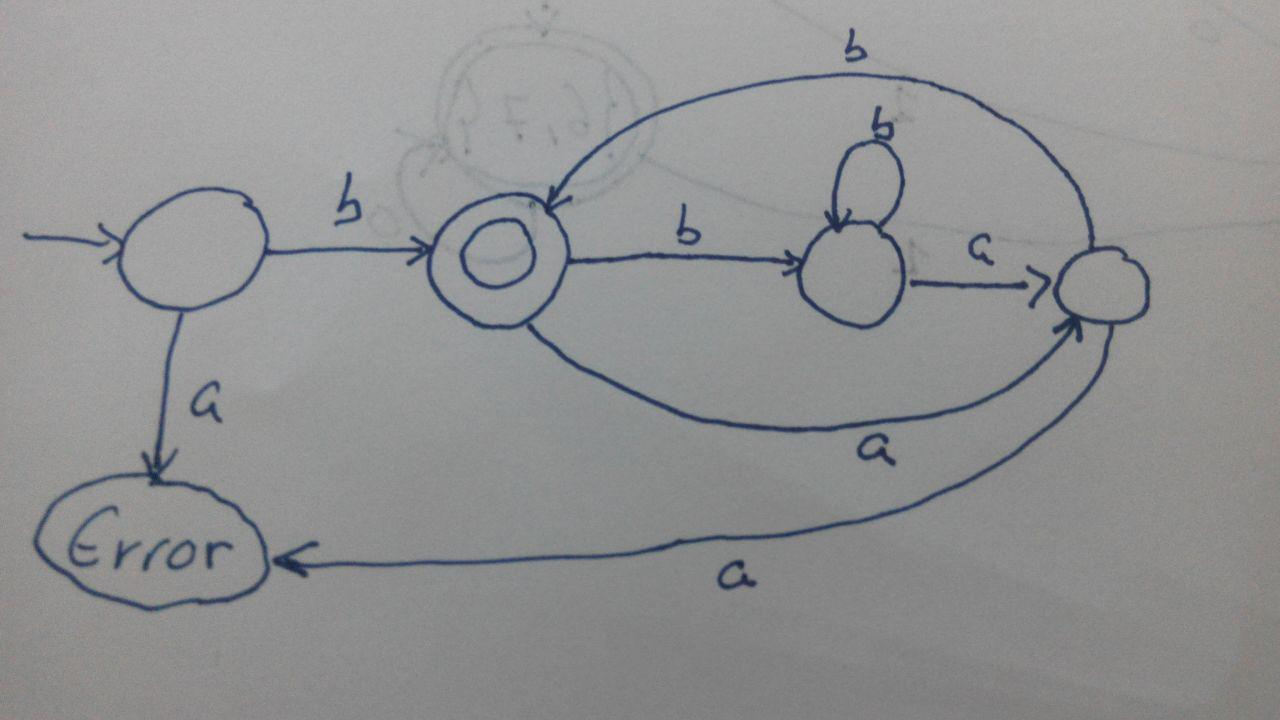
\includegraphics[width=7cm, height=5cm]{imagenes/ejercicio3b.jpg}
    \end{figure}
    \item $ (a+b)^+(ab)^+b^+ $
    \begin{figure}[H]
      \centering
      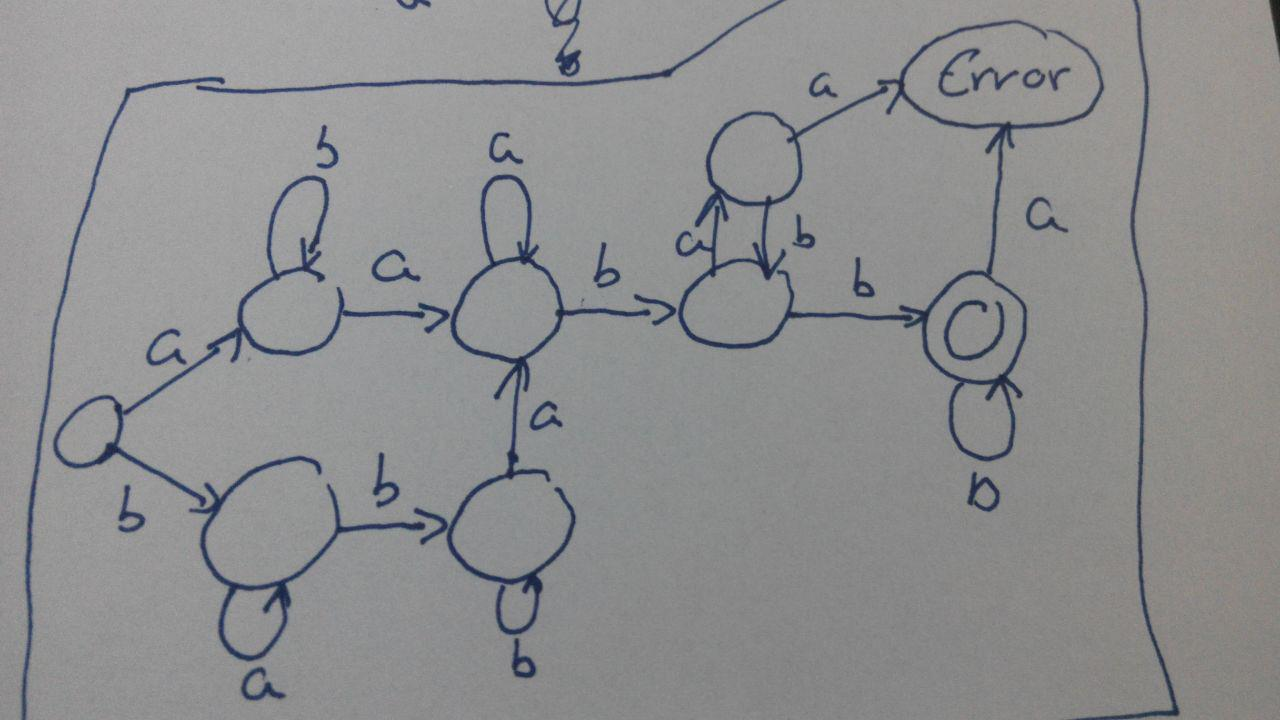
\includegraphics[width=7cm, height=5cm]{imagenes/ejercicio3c.jpg}
    \end{figure}
  \end{itemize}
\end{enumerate}
\end{document}
